\section{Diagrams}
The modeling was done in UML \cite{larman04applying} as that is the modeling language most frequently used when modeling software systems. Therefore, most people will be familiar with the models that will be presented hereafter. UML is also very suitable to model C++ code in, as most important C++ concepts have a direct counterpart in UML. All diagrams can be found in the \hyperlink{model_diagrams}{model diagrams} appendix. Once again, function references in the diagrams will be suffixed with parentheses. Perhaps the most important diagram is the one which gives a general overview of the IPC path; this diagram will now be presented.

\begin{figure}[ht]
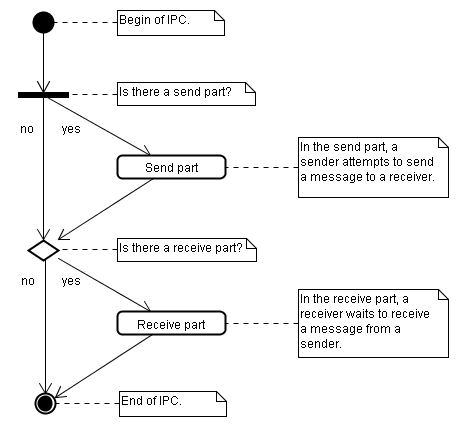
\includegraphics[scale=0.50]{images/diagrams/ipc_activity_ipc_overview}
\caption{Fiasco IPC path overview.}
\end{figure}